\documentclass[11pt]{article}
\usepackage{bookmark}
\usepackage{algorithm}
\usepackage{algpseudocode}
\usepackage{amsfonts}
\usepackage{amsmath}
\usepackage{amssymb}
\usepackage{amsthm}
\usepackage{bm}
\usepackage{color}
\usepackage{comment}
\usepackage{float}
\usepackage{graphicx}
%\usepackage[hidelinks]{hyperref}
\usepackage{makecell}
\usepackage[caption=false,font=footnotesize,subrefformat=parens,labelformat=parens]{subfig}
\usepackage{wrapfig}
\usepackage{url}
\usepackage[table]{xcolor}
\graphicspath{{images/}}
\setlength{\parindent}{0.25in}
\setlength{\parskip}{.05in}
\pagestyle{plain}
%Title, date an author of the document
\title{Progress Report}
\author{Bardia Mojra}


\begin{document}
\maketitle
\thispagestyle{empty}

\bigskip
\bigskip
\begin{center}
      Robotic Vision Lab
\end{center}

\begin{center}
      The University of Texas at Arlington
\end{center}

\newpage

\section{Specific Research Goals}
\begin{itemize}
      \item VPQEKF (April 1st): Work on the paper.
      \item DLO Manipulation Dataset (September - ICRA)
\end{itemize}

\section{To Do}
\begin{itemize}
  \item QEKF Paper (April 1st):
  \begin{itemize}
      \item Related work
      \item Introduction
      \item QuEst + VEst description
      \item QEKF description
      \item Experiments
      \item Conclusion
  \end{itemize}
  \item QEKF/DR Implementation (Feb. 2st):
  \begin{itemize}
      \item Finish updating QEKF code - done
      \item Add Vicon data as ground truth - overdue
      \item Test on multiple datasets
  \end{itemize}
  \item QEKF/QuEst+VEst Implementation (Feb. 11th):
  \begin{itemize}
      \item Integrate and confirm update QEKF works
      \item Address scale factor (depth-scale) issues
      \item Address "hand off" issue when objects enter or leave field of view
      \item Real-time streaming images for real-time operation (optional)
      \item Experiments
      \item Feature point extraction
      \item Noise issue: noise cannot be modeled
  \end{itemize}
  \item  DLO Manipulation:
  \begin{itemize}
      \item Related work literature review
      \item Real dataset + paper (September 2022 - ICRA):
      \begin{itemize}
            \item Design, discuss and build a data collection and test rig (on-going)
            \item Define DLO classes and specs
            \item Purchase DLO samples for data collection
      \end{itemize}
      \item Unity dataset
      \begin{itemize}
            \item Recreate virtual duplicates of physical test material
            \item Model dynamics and deformity
      \end{itemize}
  \end{itemize}
\end{itemize}


\section{Progress}
The following items are listed in the order of priority:
\begin{itemize}
      \item Dead Reckoning (Feb. 2nd, 2022): I debugged the DR code and was able
      to get some initial results. State estimate which is orientation in
      Quaternion seems to be noisy and highly inaccurate, see figure 1.
      With a closer examination, we suspect low observation noise on angular
      velocity might be a cause, see figure [2]. Angular velocity is measured but
      in EKF formulation, it is considered input and is a part vector \(u\).
      Dr. Gans and I suspect input signal noise \(u_Wrpy\)
      and computational errors may be
      the root causes for these issues. Thus, I am working on importing Vicon
      data to be used as ground truth. Moreover, I will try to apply a smoothing
      function
      or a moving-average filter to angular velocity signal \(u_Wrpy\) since it is
      considered input and is not expected to have noise.
      \item VPQEKF (April 1st, 2022): I need to start working on feature points
      extraction done by Quest+Vest code \cite{quest}.
      \item DLO Manipulation: I looked into getting a wiring harness assembly
      'formboard', figures 3 and 4.
      The boards are custom and are made-to-order, so we either
      have to get an old one or build one ourselves. I explained the situation
      to Dr. Gans and he said he know some senior people at GM and he is gonna
      talk to them. Additionally, I looked into a formboard stand and it costs
      about \$2,500, I will look for cheaper alternatives.
      \item NBV-Grasping Project: No update.
      \item PyTorch Tutorials: Transfer learning.
      \item Pose Estimation: I will need it for DLO segment localization.
\end{itemize}

\section{Intermediate Goals - Fall 2021:}
\begin{itemize}
      \item QEKF: Finish paper.
      \item UR5e: Do the tutorials.
\end{itemize}


\begin{figure}[h]
      \centering
      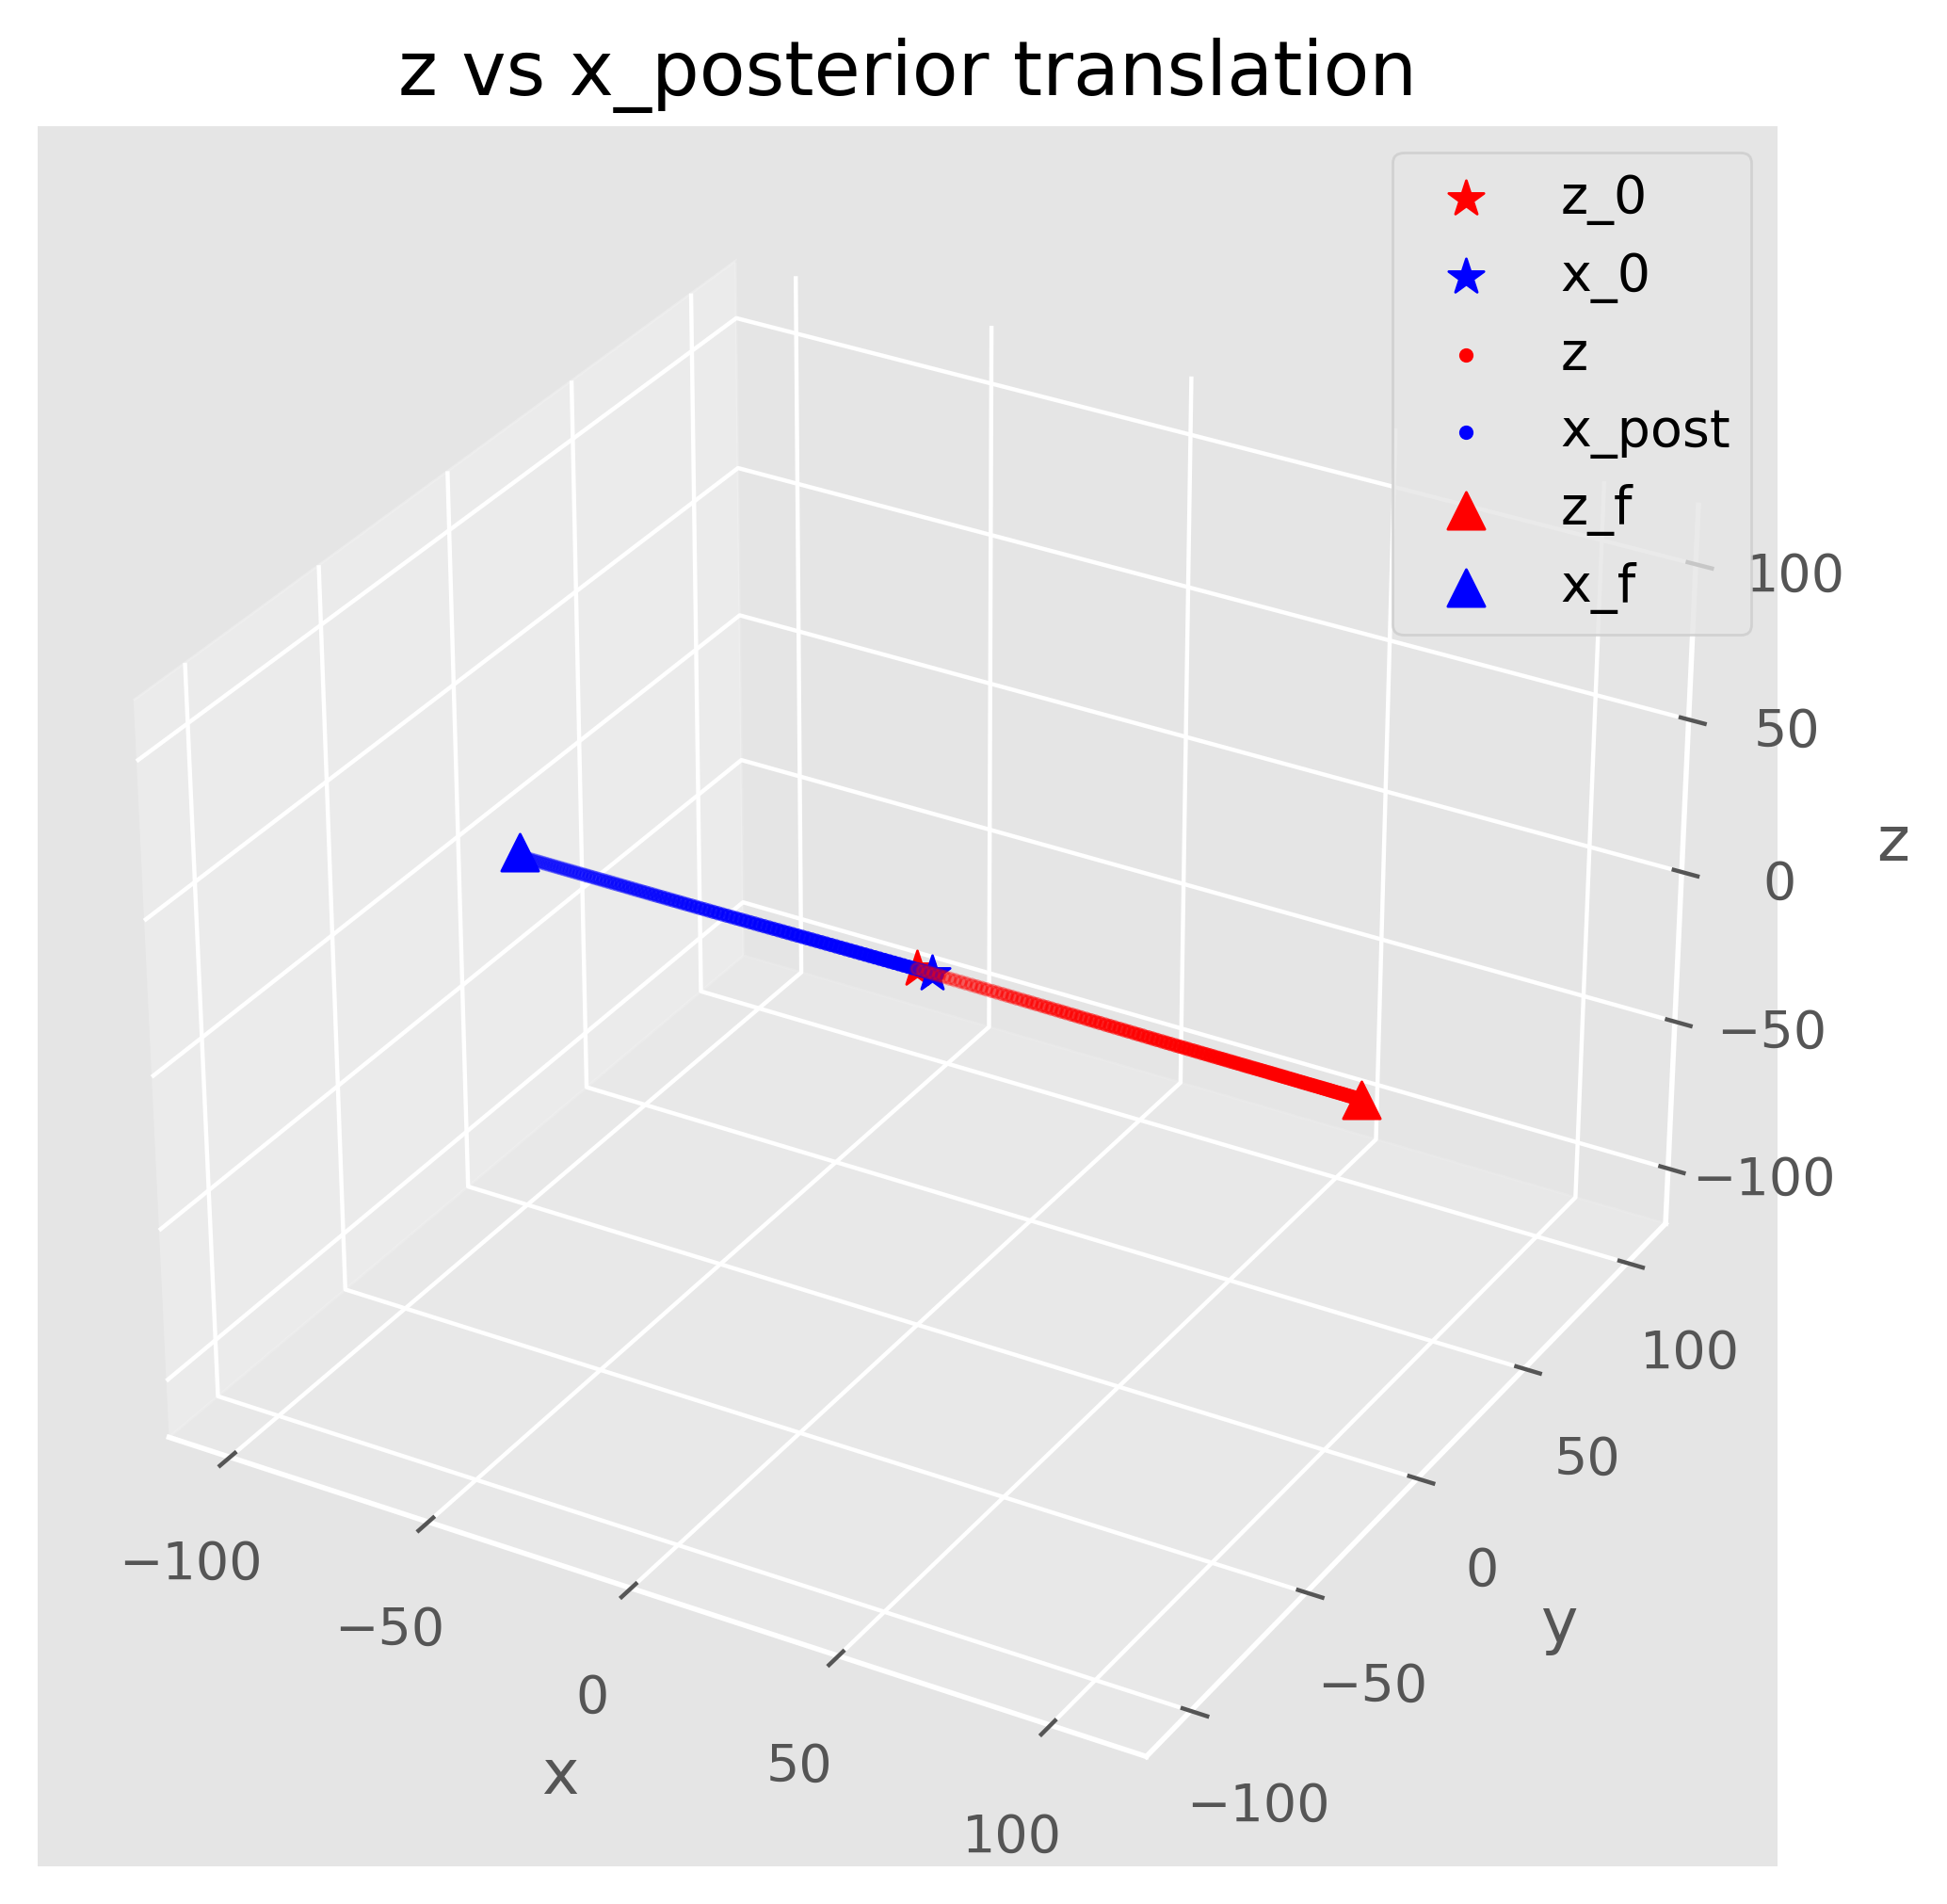
\includegraphics[width=1\textwidth]{/fig01.png}
      \caption{Measured and state estimate of orientation in Quaternion.}
\end{figure}

\begin{figure}[h]
      \centering
      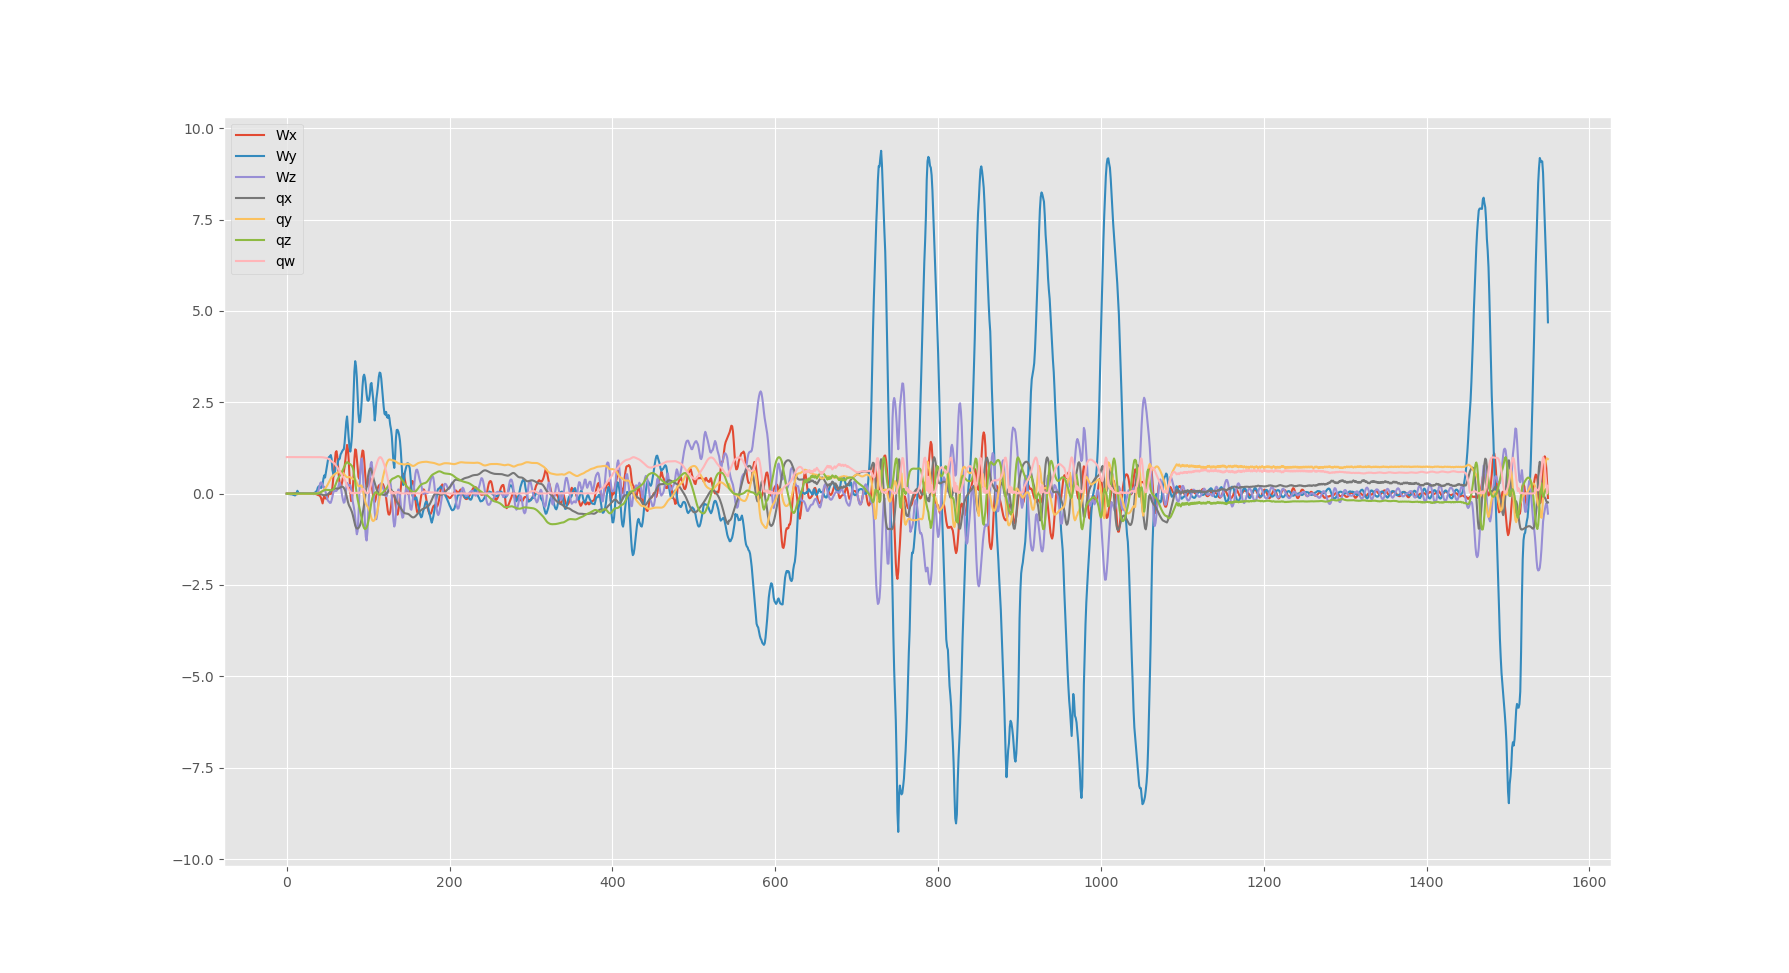
\includegraphics[width=1\textwidth]{/fig02.png}
      \caption{Input angular velocity signal and orientation state estimate in
      Quaternion.}
\end{figure}
\newpage

\begin{figure}[h]
      \centering
      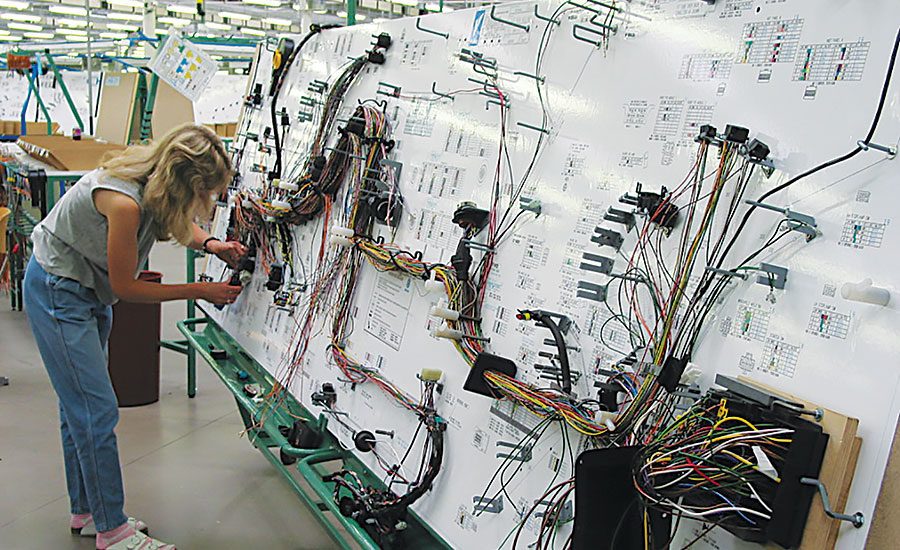
\includegraphics[width=1\textwidth]{/fig03.jpg}
      \caption{Wiring harness assembly on a designated formboard.}
\end{figure}

\begin{figure}[h]
      \centering
      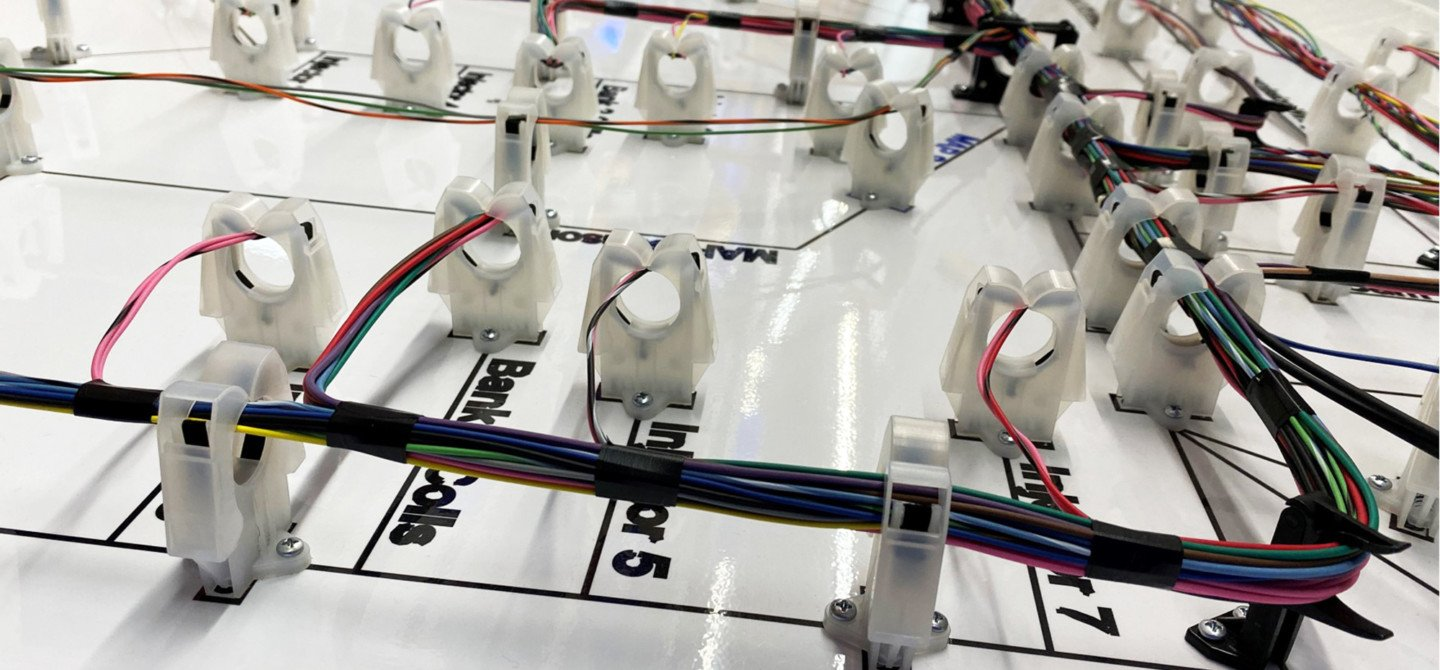
\includegraphics[width=1\textwidth]{/fig04.jpg}
      \caption{A formboard close up.}
\end{figure}
\newpage

%Sets the bibliography style to UNSRT and import the
\newpage
\bibliography{ref}
\bibliographystyle{ieeetr}

\end{document}
